%%%%%%%%%%%%%%%%%%%%%%%%%%%%%%%%%%%%%%%%%%%%%%%%%%%%%%%%%%%%%
\section{Results}

%%%%%%%%%%%%%%%%%%%%%%%%%
\begin{frame}
\frametitle{Results - Test Cases}

Test cases:
\\~

\begin{itemize}
  \item 1D manufactured:
\end{itemize}
$ \hspace{5mm} \varv{b} = \left[ 1 \right], u(x) = sin(2.15 x + 0.23), \Omega = [-1,1].$
\\~

\begin{itemize}
  \item 2D Peterson~\cite{Peterson1991}:
\end{itemize}
$ \hspace{5mm} \varv{b} = \left[ 0, 1 \right], u(x,-1) = sin(2.15 x + 0.23), \Omega = [-1,1] \times [-1,1].$

\end{frame}

%%%%%%%%%%%%%%%%%%%%%%%%%
\begin{frame}
\frametitle{Results - Discrete Spaces}

DPG:
\begin{alignat}{3}
& \fspace{U}_h = \{ \varv{u} \coloneqq (u,f^*) && : u \in \fspace{L}^2(\fspace{\Omega}), u|_{\fe{V}} \in \mathcal{P}^{p}\ \forall \fe{V}, \\
                                             &  && : f^* \in \fspace{L}^2(\fspace{\Omega}), f^*|_{\fe{F}} \in \mathcal{P}^\makered{p+1}\ \forall \fe{F} \}. \\
& \fspace{V}_h = \{ v && : v \in \fspace{L}^2(\fspace{\Omega}), v|_{\fe{V}} \in \mathcal{P}^{p+2}\ \forall \fe{V} \}.
\end{alignat}

OPG:
\begin{alignat}{3}
& \fspace{U}_h = \{ u && : u \in \fspace{L}^2(\fspace{\Omega}), u|_{\fe{V}} \in \mathcal{P}^{p}\ \forall \fe{V} \}. \\
& \fspace{V}_h = \{ v && : v \in \fspace{C}^0(\fspace{\Omega}), v|_{\fe{V}} \in \mathcal{P}^{\makered{p+1}\ (\text{or}\ p)}\ \forall \fe{V} \}.
\end{alignat}

DG:
\begin{alignat}{3}
& \fspace{U}_h = \{ u && : u \in \fspace{L}^2(\fspace{\Omega}), u|_{\fe{V}} \in \mathcal{P}^{p}\ \forall \fe{V} \}. \\
& \fspace{V}_h = \{ v && : v \in \fspace{L}^2(\fspace{\Omega}), v|_{\fe{V}} \in \mathcal{P}^{p}\ \forall \fe{V} \}.
\end{alignat}

\end{frame}

%%%%%%%%%%%%%%%%%%%%%%%%%%%%%%%%%%%%%%%%%%%%%%%%%%%%%%%%%%%%%
\subsection{1D Manufacatured}

%%%%%%%%%%%%%%%%%%%%%%%%%
\begin{frame}
\frametitle{Manufactured - Convergence Rates}

\begin{table}[!ht]
\begin{center}
\caption{Convergence Orders - 1D Manufactured Solution}
% \resizebox{\textwidth}{!}{
\resizebox{\textwidth}{\dimexpr0.9\textheight-5.5cm\relax}{
\begin{tabular}{| l | c | c c c c c | }
	\hline
	\multicolumn{2}{|c|}{} & \multicolumn{5}{c|}{Conv. Order} \\
	\hline
	Order ($p$) & Mesh Size ($h$) & $L^2 (u)_{L^2}$ & $L^2 (u)_{\text{OPG}}$ & $L^2 (u)_{\text{DPG} - H_b^1}$ & $L^2 (u)_{\text{DPG} - H_b^-}$ & $L^2 (u)_{\text{DG}}$ \\
	\hline
0	& 2.50e-01 & -    & -    & -    & -    & -    \\
	& 1.25e-01 & 0.95 & -    & 0.98 & 0.98 & 1.08 \\
	& 6.25e-02 & 0.99 & -    & 1.06 & 1.06 & 1.04 \\
	\hline
1	& 1.25e-01 & -    & -    & -    & -    & -    \\
	& 6.25e-02 & 2.00 & 2.00 & 2.14 & 2.14 & 2.00 \\
	& 3.12e-02 & 2.00 & 2.00 & 2.06 & 2.06 & 2.00 \\
	\hline
2	& 8.33e-02 & -    & -    & -    & -    & -    \\
	& 4.17e-02 & 2.96 & 2.96 & 2.95 & 2.95 & 2.99 \\
	& 2.08e-02 & 2.99 & 2.99 & 3.01 & 3.01 & 3.00 \\
	\hline
\end{tabular}
}
\end{center}
\end{table}

\end{frame}

%%%%%%%%%%%%%%%%%%%%%%%%%
\begin{frame}
\frametitle{Manufactured - Errors}

\begin{table}[!ht]
\begin{center}
\caption{Errors - 1D Manufactured Solution}
% \resizebox{\textwidth}{!}{
\resizebox{\textwidth}{\dimexpr0.9\textheight-5.5cm\relax}{
\begin{tabular}{| l | c | c c c c c | }
	\hline
	\multicolumn{2}{|c|}{} & \multicolumn{5}{c|}{$L^2$ Error} \\
	\hline
	Order ($p$) & Mesh Size ($h$) & $L^2 (u)_{L^2}$ & $L^2 (u)_{\text{OPG}}$ & $L^2 (u)_{\text{DPG} - H_b^1}$ & $L^2 (u)_{\text{DPG} - H_b^-}$ & $L^2 (u)_{\text{DG}}$ \\
	\hline
0	& 2.50e-01 & 1.89e-01 & -    & 2.22e-01 & 2.21e-01 & 3.80e-01 \\
	& 1.25e-01 & 9.77e-02 & -    & 1.13e-01 & 1.12e-01 & 1.80e-01 \\
	& 6.25e-02 & 4.92e-02 & -    & 5.40e-02 & 5.40e-02 & 8.76e-02 \\
	\hline
1	& 1.25e-01 & 3.33e-02 & 3.33e-02 & 3.98e-02 & 3.98e-02 & 4.27e-02 \\
	& 6.25e-02 & 8.31e-03 & 8.31e-03 & 9.01e-03 & 9.01e-03 & 1.07e-02 \\
	& 3.12e-02 & 2.08e-03 & 2.08e-03 & 2.15e-03 & 2.15e-03 & 2.67e-03 \\
	\hline
2	& 8.33e-02 & 2.39e-03 & 2.39e-03 & 2.46e-03 & 2.46e-03 & 2.92e-03 \\
	& 4.17e-02 & 3.08e-04 & 3.08e-04 & 3.19e-04 & 3.19e-04 & 3.69e-04 \\
	& 2.08e-02 & 3.88e-05 & 3.88e-05 & 3.97e-05 & 3.97e-05 & 4.61e-05 \\
	\hline
\end{tabular}
}
\end{center}
\end{table}

\end{frame}

%%%%%%%%%%%%%%%%%%%%%%%%%%%%%%%%%%%%%%%%%%%%%%%%%%%%%%%%%%%%%
\subsection{2D Peterson}

%%%%%%%%%%%%%%%%%%%%%%%%%
\begin{frame}
\frametitle{Peterson - Convergence Rates}

\begin{table}[!ht]
\begin{center}
\caption{Convergence Orders - Peterson Meshes}
% \resizebox{\textwidth}{!}{
\resizebox{\textwidth}{\dimexpr0.9\textheight-5.5cm\relax}{
\begin{tabular}{| l | c | c c c c c | }
	\hline
	\multicolumn{2}{|c|}{} & \multicolumn{5}{c|}{Conv. Order} \\
	\hline
	Order ($p$) & Mesh Size ($h$) & $L^2 (u)_{L^2}$ & $L^2 (u)_{\text{OPG}}$ & $L^2 (u)_{\text{DPG} - H_b^1}$ & $L^2 (u)_{\text{DPG} - H_b^-}$ & $L^2 (u)_{\text{DG}}$ \\
	\hline
0	& 1.12e-01 & -    & -    & -    & -    & -    \\
	& 5.74e-02 & 0.91 & -    & 1.04 & 0.96 & 0.32 \\
	& 2.95e-02 & 1.01 & -    & 1.10 & 1.14 & 0.51 \\
	& 1.49e-02 & \makeblue{1.00} & -    & \makeblue{0.99} & \makeblue{1.05} & \makered{0.50} \\
	\hline
1	& 6.15e-02 & -    & -    & -    & -    & -    \\
	& 3.15e-02 & 2.10 & 1.18 & 2.19 & 2.18 & 1.74 \\
	& 1.61e-02 & 2.00 & 1.05 & 1.90 & 2.02 & 1.42 \\
	& 8.22e-03 & \makeblue{2.02} & \makeblue{1.04} & \makeblue{2.23} & \makeblue{2.30} & \makered{1.50} \\
	\hline
2	& 4.35e-02 & -    & -    & -    & -    & -    \\
	& 2.18e-02 & 2.81 & 2.11 & 2.90 & 2.96 & 2.47 \\
	& 1.11e-02 & 3.05 & 1.94 & 3.12 & 3.13 & 2.56 \\
	& 5.64e-03 & 3.01 & \makeblue{2.01} & 3.02 & 3.00 & \makered{2.62} \\
	\hline
\end{tabular}
}
\end{center}
\end{table}

\end{frame}


%%%%%%%%%%%%%%%%%%%%%%%%%
\begin{frame}
\frametitle{Peterson - Errors}

\begin{table}[!ht]
\begin{center}
\caption{$L^2$ Errors - Peterson Meshes}
% \resizebox{\textwidth}{!}{
\resizebox{\textwidth}{\dimexpr0.9\textheight-5.5cm\relax}{
\begin{tabular}{| l | c | c c c c c | }
	\hline
	\multicolumn{2}{|c|}{} & \multicolumn{5}{c|}{$L^2$ Error} \\
	\hline
	Order ($p$) & Mesh Size ($h$) & $L^2 (u)_{L^2}$ & $L^2 (u)_{\text{OPG}}$ & $L^2 (u)_{\text{DPG} - H_b^1}$ & $L^2 (u)_{\text{DPG} - H_b^-}$ & $L^2 (u)_{\text{DG}}$ \\
	\hline
0	& 1.12e-01 & 1.19e-01 & -    & 1.49e-01 & 1.82e-01 & 2.26e-01 \\
	& 5.74e-02 & 6.49e-02 & -    & 7.43e-02 & 9.61e-02 & 1.83e-01 \\
	& 2.95e-02 & 3.32e-02 & -    & 3.58e-02 & 4.49e-02 & 1.31e-01 \\
	& 1.49e-02 & 1.69e-02 & -    & 1.83e-02 & 2.20e-02 & 9.29e-02 \\
	\hline
1	& 6.15e-02 & 1.66e-02 & 1.60e-01 & 2.24e-02 & 2.63e-02 & 4.48e-02 \\
	& 3.15e-02 & 4.06e-03 & 7.23e-02 & 5.17e-03 & 6.10e-03 & 1.39e-02 \\
	& 1.61e-02 & 1.07e-03 & 3.59e-02 & 1.46e-03 & 1.58e-03 & 5.39e-03 \\
	& 8.22e-03 & \makeblue{2.74e-04} & 1.77e-02 & \makeblue{3.23e-04} & \makeblue{3.35e-04} & 1.96e-03 \\
	\hline
2	& 4.35e-02 & 8.79e-04 & 1.97e-02 & 1.75e-03 & 1.81e-03 & 2.11e-03 \\
	& 2.18e-02 & 1.25e-04 & 4.55e-03 & 2.34e-04 & 2.32e-04 & 3.81e-04 \\
	& 1.11e-02 & 1.62e-05 & 1.24e-03 & 2.90e-05 & 2.85e-05 & 6.85e-05 \\
	& 5.64e-03 & 2.09e-06 & \makeblue{3.16e-04} & 3.71e-06 & 3.71e-06 & 1.15e-05 \\
	\hline
\end{tabular}
}
\end{center}
\end{table}

\end{frame}

%%%%%%%%%%%%%%%%%%%%%%%%%%%%%%%%%%%%%%%%%%%%%%%%%%%%%%%%%%%%%
\subsection{Discussion}

%%%%%%%%%%%%%%%%%%%%%%%%%
\begin{frame}
\frametitle{Overconstrained Space for OPG}

Visualization of converged solution for a two dimensional manufactured solution:

\newcommand*{\figurepath}{../manuscript/figures}%
\begin{figure}[!h]
    \centering
    \begin{subfigure}{0.485\textwidth}
        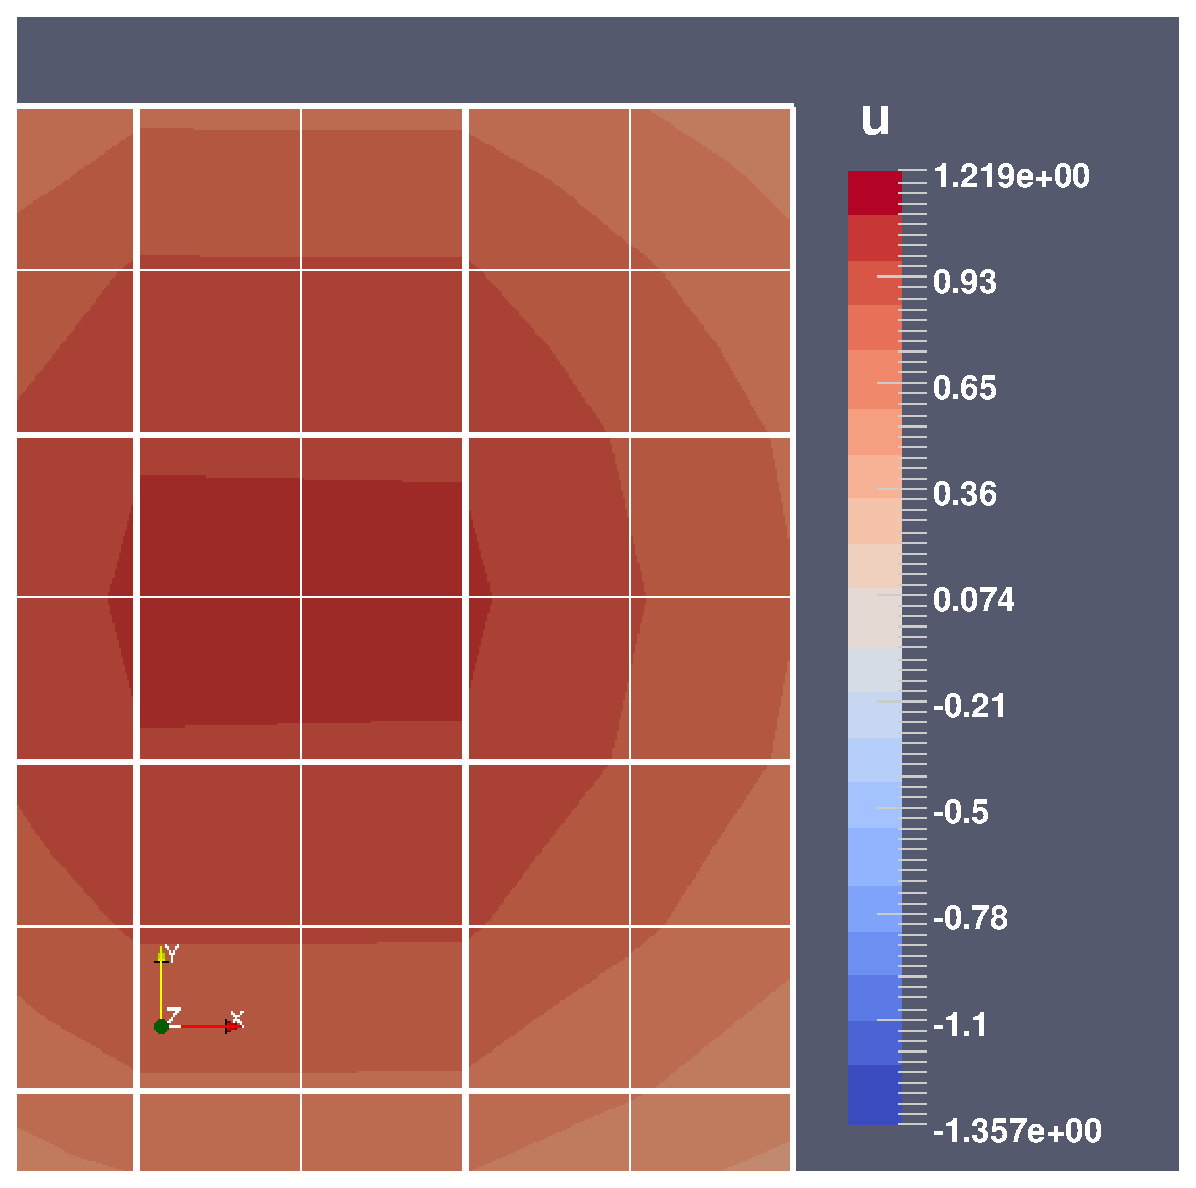
\includegraphics[width=\textwidth]{./results/data/manufactured_2d/opgc_man_2d_bx.eps}
        \caption{$\varv{b} = [1,0]$}
    \end{subfigure}
\hfill
    \begin{subfigure}{0.485\textwidth}
        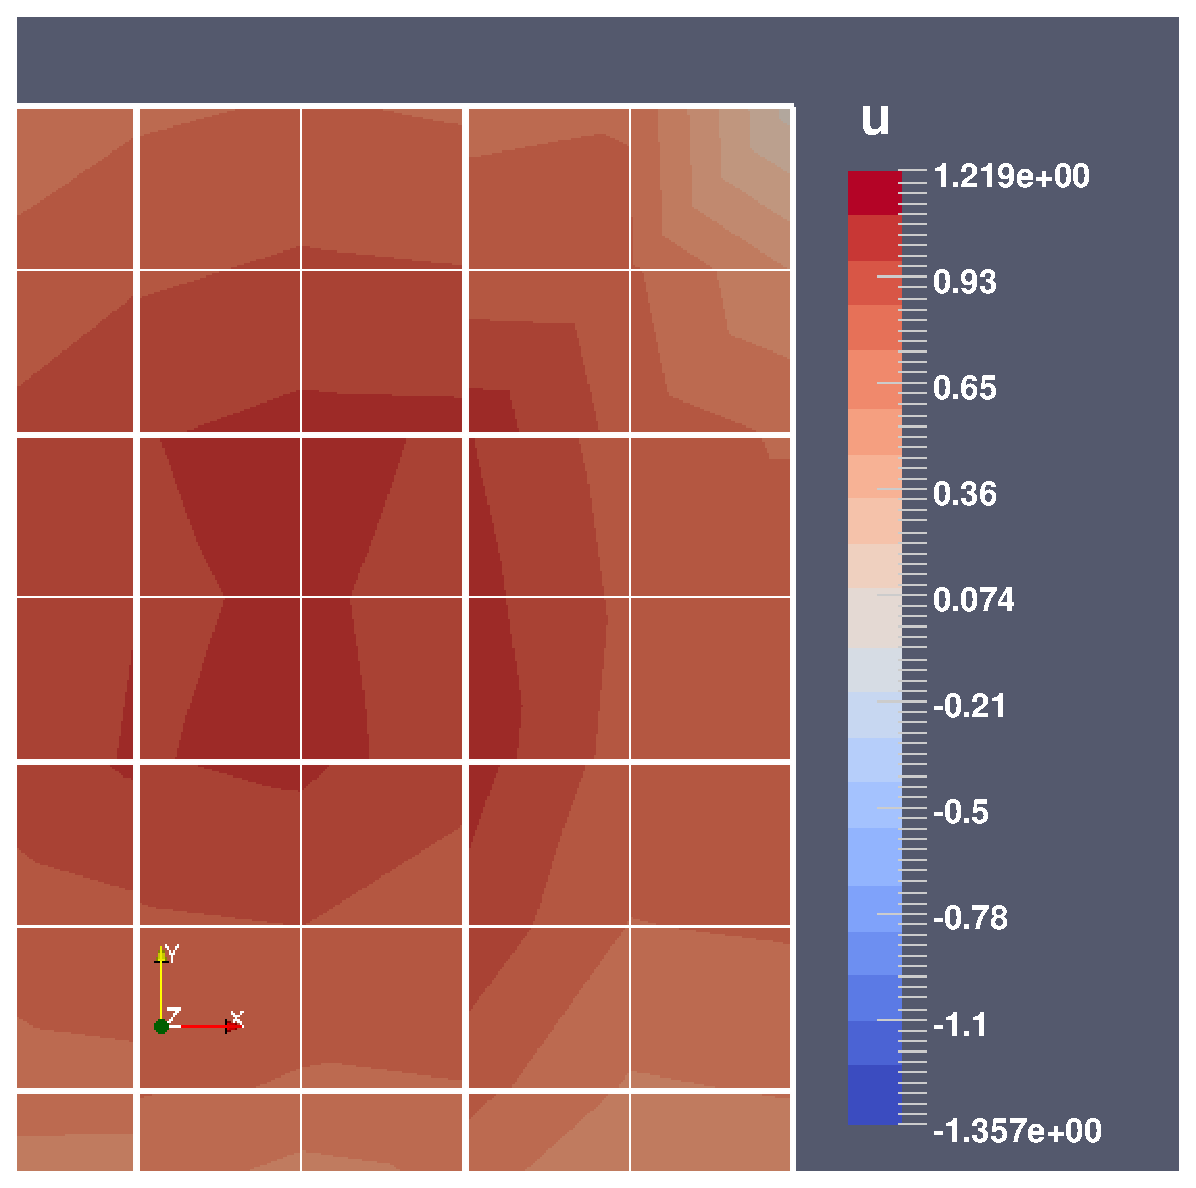
\includegraphics[width=\textwidth]{./results/data/manufactured_2d/opgc_man_2d_bxy.eps}
        \caption{$\varv{b} = [0.23,0.45]$}
    \end{subfigure}
\caption{Overconstrained Test Space with Multiple Outflow Faces}
\end{figure}

\end{frame}